\documentclass[12pt,a4paper]{article}
\usepackage[utf8]{inputenc}
\usepackage[T1]{fontenc}
\usepackage[francais]{babel}
\usepackage{amsmath}
\usepackage{amsfonts}
\usepackage{amssymb}
\usepackage{graphicx}
\usepackage[top=2.00cm]{geometry}
\usepackage{titlesec}
\usepackage{epstopdf}
\usepackage{bigcenter}
%%modif des titres de section diminuer la taille
\renewcommand{\thesection}{\Roman{section}}
\titleformat{\section}
{\normalfont\bfseries\Large\scshape}{\thesection}{1em}{}
\titleformat{\subsection}
{\normalfont\bfseries\large}{\thesubsection}{1em}{}
\graphicspath{{./res/}}
\makeatletter
\def\@maketitle{

	\begin{center}
	% NoLogo
	%	\vspace*{+2cm}
	
	%	Corner Logo
	%	\begin{flushright}
	%		
\includegraphics[width=40mm]{logo_corner}\\[4ex]
	%	\end{flushright}
	
	%	Top Logo
		
\includegraphics[scale=0.3]{res/logo_top}

			
				{\LARGE \@title }\\[4ex]
				{\large \@author}\\[4ex]
				{\large \@date}\\[8ex]
		\rule{\linewidth}{0.4pt}
	\end{center}
}
\makeatletter

\author{CHARNAY Valentin, FINOT Sylvain, LEE Mijin}
\title{Compte rendu de TP :\\[4pt] \scshape Analyse de Fourier d'ondes sonores}

\date{\today}
\begin{document}
\maketitle
Dans ce TP, nous avons étudié et analysé des ondes sonores de différentes fréquences (noté $\nu$).
\section*{Conversion numérique d'un signal analogique}

\section*{Analyse de la résonance dans un tube}
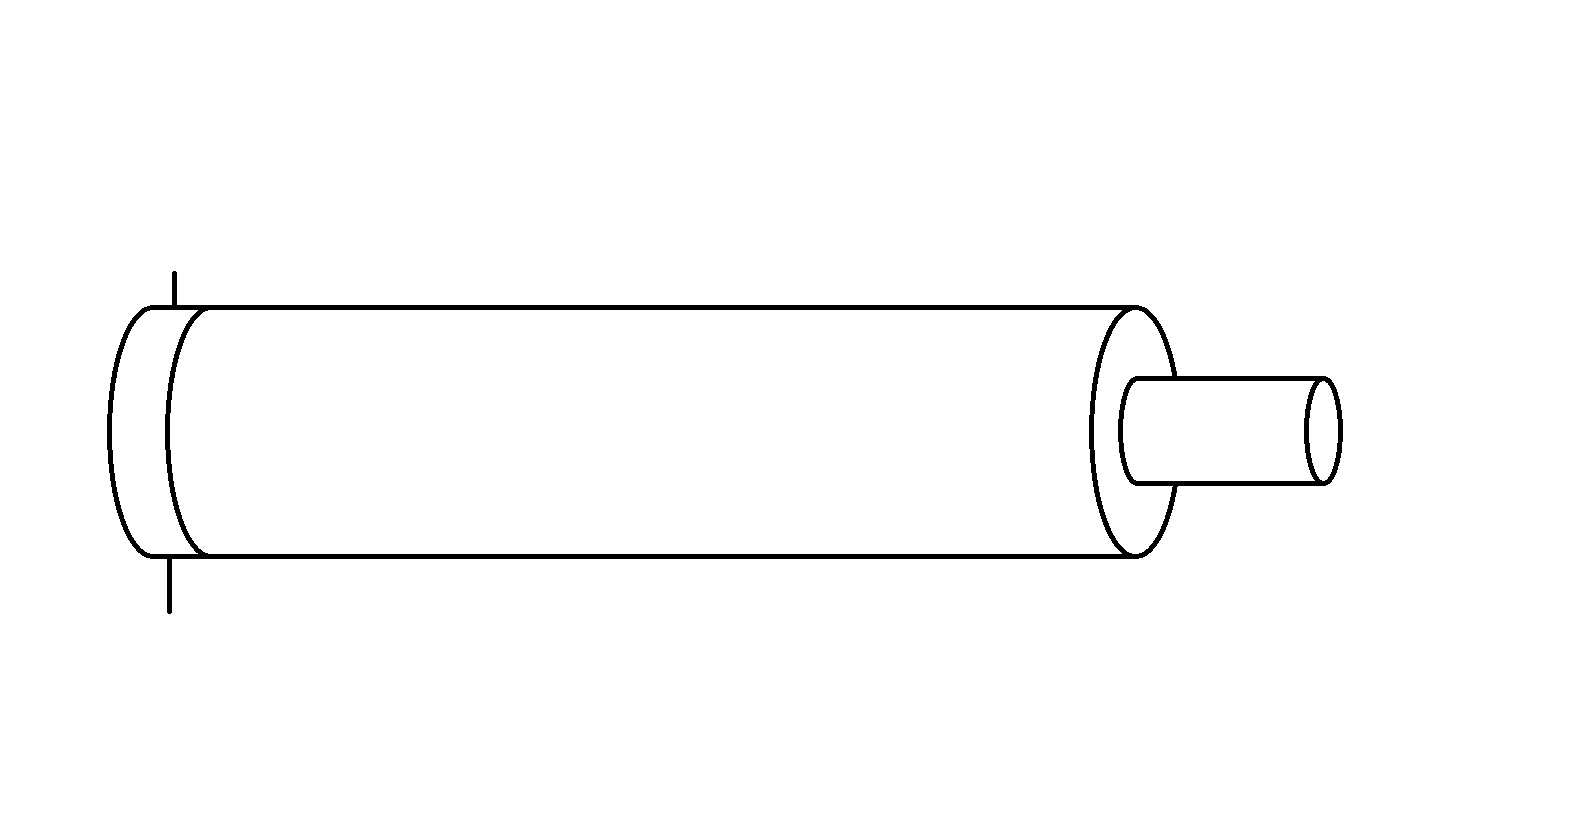
\includegraphics[scale=0.5]{schetub1}
\section{bordel}
\begin{bigcenter}
		\includegraphics[width=1.5\linewidth]{"Resonance tuyau a vide"}			
\end{bigcenter}
\begin{figure}
	\centering
	\includegraphics[width=0.7\linewidth]{"res/Resonance tuyau PVC mou"}
	\caption{}
	\label{fig:resonance-tuyau-pvc-mou}
\end{figure}
\begin{figure}
	\centering
	\includegraphics[width=0.7\linewidth]{"res/Resonance tuyau PVC rigide"}
	\caption{}
	\label{fig:resonance-tuyau-pvc-rigide}
\end{figure}
\begin{figure}
	\centering
	\includegraphics[width=0.7\linewidth]{"res/Valentin aigu"}
	\caption{}
	\label{fig:valentin-aigu}
\end{figure}
\begin{figure}
	\centering
	\includegraphics[width=0.7\linewidth]{"res/Valentin grave"}
	\caption{}
	\label{fig:valentin-grave}
\end{figure}
\begin{figure}
	\centering
	\includegraphics[width=0.7\linewidth]{"res/diapason casse"}
	\caption{}
	\label{fig:diapason-casse}
\end{figure}
\begin{figure}
	\centering
	\includegraphics[width=0.7\linewidth]{"res/diapason repare"}
	\caption{}
	\label{fig:diapason-repare}
\end{figure}
\begin{figure}
	\centering
	\includegraphics[width=0.7\linewidth]{"res/echantillonnage 200Hz"}
	\caption{}
	\label{fig:echantillonnage-200hz}
\end{figure}
\begin{figure}
	\centering
	\includegraphics[width=0.7\linewidth]{"res/echantillonnage 400Hz"}
	\caption{}
	\label{fig:echantillonnage-400hz}
\end{figure}
\begin{figure}
	\centering
	\includegraphics[width=0.7\linewidth]{"res/echantillonnage 500Hz"}
	\caption{}
	\label{fig:echantillonnage-500hz}
\end{figure}
\begin{figure}
	\centering
	\includegraphics[width=0.7\linewidth]{"res/echantillonnage 1000Hz"}
	\caption{}
	\label{fig:echantillonnage-1000hz}
\end{figure}
\begin{figure}
	\centering
	\includegraphics[width=0.7\linewidth]{"res/echantillonnage 2000Hz"}
	\caption{}
	\label{fig:echantillonnage-2000hz}
\end{figure}
\begin{figure}
	\centering
	\includegraphics[width=0.7\linewidth]{"res/echantillonnage 3000Hz"}
	\caption{}
	\label{fig:echantillonnage-3000hz}
\end{figure}
\begin{figure}
	\centering
	\includegraphics[width=0.7\linewidth]{"res/echantillonnage 4000Hz"}
	\caption{}
	\label{fig:echantillonnage-4000hz}
\end{figure}
\begin{figure}
	\centering
	\includegraphics[width=0.7\linewidth]{"res/echantillonnage 10000Hz"}
	\caption{}
	\label{fig:echantillonnage-10000hz}
\end{figure}
\begin{figure}
	\centering
	\includegraphics[width=0.7\linewidth]{"res/guitare 0"}
	\caption{}
	\label{fig:guitare-0}
\end{figure}
\begin{figure}
	\centering
	\includegraphics[width=0.7\linewidth]{"res/guitare 1"}
	\caption{}
	\label{fig:guitare-1}
\end{figure}
\begin{figure}
	\centering
	\includegraphics[width=0.7\linewidth]{"res/guitare 2"}
	\caption{}
	\label{fig:guitare-2}
\end{figure}
\begin{figure}
	\centering
	\includegraphics[width=0.7\linewidth]{"res/Noemie grave"}
	\caption{}
	\label{fig:noemie-grave}
\end{figure}
\begin{figure}
	\centering
	\includegraphics[width=0.7\linewidth]{"res/Resonance tuyau a vide"}
	\caption{}
	\label{fig:resonance-tuyau-a-vide}
\end{figure}
\begin{figure}
	\centering
	\includegraphics[width=0.7\linewidth]{"res/Resonance tuyau bois"}
	\caption{}
	\label{fig:resonance-tuyau-bois}
\end{figure}
\begin{figure}
	\centering
	\includegraphics[width=0.7\linewidth]{"res/Resonance tuyau polystyrene"}
	\caption{}
	\label{fig:resonance-tuyau-polystyrene}
\end{figure}



\end{document}
